\documentclass[12pt,a4paper]{report}
\synctex=1
\usepackage[utf8]{inputenc}
\usepackage[margin=2cm, top=1.5cm, bottom=2cm]{geometry}

\usepackage{graphicx}
\usepackage{libertine}
\usepackage{amsmath}
\usepackage{amssymb}
\usepackage{listings}
\usepackage{pgfornament}
\usepackage{eso-pic}
\usepackage{textcomp}
\usepackage{courier}
\usepackage[hangul]{kotex}
\usepackage{rotating}
\usepackage{dirtree}

\title{
	\centering
	\pgfornament[width=12cm,color=teal]{84}\\
	\vspace{1cm}
	\fontsize{50}{50} \selectfont {오목 인공지능 형성\\설계과제 최종 보고서}\\
		\pgfornament[width=12cm,color=teal]{88}\\
	\vfill}
\author{
	\LARGE
	\begin{tabular}{rl}
		\hline
		교과목명 : & 자료구조와 실습\\
		담당교수 : & 정 준호 교수님\\
		프로젝트명 : & $ \Omega $目\\
		학번 : & 2016110056\\ 
		이름 : & 박승원\\
		날짜 : & \today\\
		\hline
	\end{tabular}\vspace{1cm}
	\\

\includegraphics[width=0.5\textwidth]{logo.jpg}
	}
\date{}


\linespread{1.3}

\begin{document}

\maketitle

%\includegrap

\newpage
\tableofcontents
\newpage
\chapter*{과제 요약서}
\paragraph{설계 과제명} 학습형 오목 인공지능 형성\\ 
\paragraph{주요기술용어} 인공지능, Machine Learning, 오목, 해싱, 이진트리\\
\paragraph{1. 과제목표} 오목 게임의 기초적인 룰만을 바탕으로 컴퓨터끼리의 대국을 통하여 실력을 늘려나가는 학습형 인공지능을 형성한다.\\
\paragraph{2. 수행 내용 및 방법} C를 이용하여 Makefile 프로젝트로  프로그램 작성\\
\paragraph{3. 수행 결과} 어느 정도 사람과 두어볼 수 있는 오목 인공지능이 형성되었으나, 매우 엉뚱한 수를 두는 경우도 있었다. 
\paragraph{4. 결과 분석} 실제로 오목 게임의 경우의 수는 매우 방대해서, 예상한 것과는 달랐다. 오목이 단순한 것은 알고리즘 측면에서의 얘기이지 경우의 수가 작은 것은 아니라는 것을 느꼈다.\\

\noindent
\chapter{서론}
\section{설계과제 목적}
\begin{itemize}
\item 창의적 사고 및 다양한 방법을 통한 문제 해결 능력
\item 여러 가지 제약조건을 고려한 효율적인 프로그램 설계 능력
\end{itemize}
\section{설계과제 내용}
머신 러닝을 기반으로 한 오목 게임용 학습형 인공 지능을 형성한다.

\section{진행일정 및 개인별 담당 분야}
독자 프로젝트임.

\begin{tabular}{|c|c|}
	\hline
	세부 개발내용&주별 세부 추진 일정\\
	\hline
	자료수집 및 설계 계획 수립&$\sim$ 11/16\\
	요구사항 검토&11.17\\
	구조도 및 모듈 설계&11.18\\
	프로그램 설계&11.19\\
	프로그램 코딩&11.20$\sim$ 11.25\\
	성능확인 및 오류 수정&11.26\\
	최종 점검 및 개선 사항 보완&11.27\\
	\hline
\end{tabular}
\chapter{프로그램의 구조 및 구성}

\section{전체 구성도}
오목판은 20X20의 캐릭터 배열로 구성한다.
흑은 X로 백은 O로 표현한다.
매번 둘 때마다 컴퓨터는 기보와 그 기보에서 자신이 둔 위치를 저장한다.

그림 \ref{data}에서 바둑판은 우선 압축 알고리즘에 의해 숫자로 7,-1,1,-4로 변환된다.
이는 단순히 바둑판의 첫칸부터 세어서 바둑돌이 나오는 순간까지의 빈칸의 숫자에 흑일 경우 +, 백일 경우 -를 붙인 것이다.
단순한 알고리즘이지만, 압축률은 OX캐릭터를 저장할 때보다 4배에서 20배 가량 높았다.

이렇게 압축한 데이터를 그 자료의 길이에 따라서 해시하여 이진트리에 저장한다.
이진트리는 그 기보에서 둘 수 있는 위치를 다시 배열로 가지고 있다.
위의 오목판에서 X표시를 한 부분은 이 기보에서 컴퓨터가 둔 위치이다. 
그 위치에 해당하는 곳에 최종 승패가 판 가름날 때에 승패의 결과를 누적한다.

이렇게 누적한 결과를 바탕으로 인간과 대결시에 승률을 계산하여 오목을 두는 인공지능을 형성한다.
\begin{sidewaysfigure}
	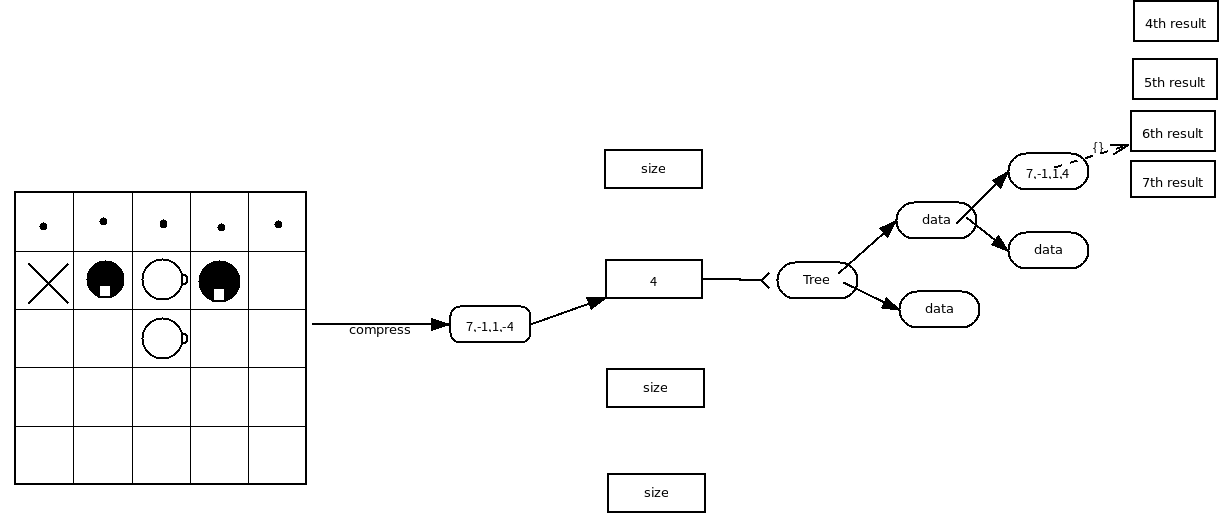
\includegraphics[width=\textwidth]{1.png}
	\caption{자료구조 도해}
	\label{data}
\end{sidewaysfigure}

\newpage
\section{프로그램 세부 구성}
\subsection{Tree 구조와 파일}

\dirtree {%
.1 root.
.3 Makefile : 하위 디렉토리의 Makefile들을 실행시킴.
.2 src. 
.3 Makefile.
.3 om.c : main함수.
.3 board.c.
.3 ai.c : 핵심적인 인공지능 모듈.
.3 find.c : 오목에서 승리점과 결정적인 지점을 찾는 함수.
.3 tree.c : tree 모듈.
.3 file.c : 기보들을 파일로 저장하는 모듈.
.3 queue.c : find.c에서 사용하는 큐.
.3 queue.h.
.3 compress.c : 오목판을 압축하고 해제하는 함수.
.2 obj.
.3 Makefile : obj파일들을 링크하는 역할.	
}

\subsection{AI 모듈 설명(ai.c)}
\subsubsection{Oai()}

\paragraph{check()} 현재 기보에서 둘 수 있는 위치를 v 표시한다.
\paragraph{put(int n)} v 표시 한 것 중에서 n번째에 둔다.
\paragraph{record()} 현 상태의 기보를 저장한다.
\paragraph{win()} 한 게임이 종료되면 그 게임에서 저장된 기보들에 승패의 결과를 기록한다.

\subsubsection{OH(), 사람과 대전시의 AI}
Oai함수와 동일한 루틴을 거치다가 수를 결정할 때에 기보 데이터를 뒤진다.
\paragraph{pre\_cog()}
기보 데이터가 없을 때에 현재의 기보 상황을 시작점으로 100판을 컴퓨터끼리 두어서 동적으로 기보를 생성한다.

\subsubsection{Xai()}
Oai함수와 동일.

\chapter{결과 및 토의}
기보의 데이터가 방대하여 오목이 알고리즘적으로 접근했을 때에 간단하단 것이지, 경우의 수가 적은 것은 아니었다.
10000판을 컴퓨터끼리 대전하게 했더니 약 20분이 걸렸다.
메모리를 1기가를 잡아먹고 생성한 기보파일도 900메가 바이트에 달했으나, 승패 결과 누적을 한 데이터 파일은 아직도 대부분이 빈 칸이었다.
처음 몇 수는 경우의 수가 적어서 데이터가 충분히 누적되었으나 3수만 지나면, 이미 백만판 이상은 둬야 어느 정도 데이터가 생성될 것 같았다.
\\

처음 수의 경우 누적된 승패\\
 0 3 0 9 0 24 0 -83 0 \\
 383 155 385 169 373 137 383 138 355 162 391 137 357 152 392 121 323 190 322 156 458 140 401 140 425 149 364 129 363 141 363 144 409 131 390 164 364 137 414 143 368 123 413 137 330 166 394 150 
\\

두 수 이후의 텅빈 데이터치\\
0 5 0 37 0 40 0 65 -18 -20 0 \\
0 0 0 1 1 0 0 0 0 0 0 0 0 0 0 0 1 0 0 0 0 0 1 0 0 0 0 0 0 0 0 0 0 0 0 0 1 0 0 1 0 0 0 0 0 0 0 0 1 0 0 1 0 0 0 0 0 0 0 0 0 1 0 0 0 0 1 0 1 0 1 0 1 0 1 1 0 1 0 0 \\
0 5 0 34 0 36 0 64 -1 -18 0 \\
0 0 0 0 0 0 0 0 0 0 0 0 0 0 0 0 0 0 0 0 1 0 0 0 0 0 0 0 0 0 0 0 0 0 0 0 0 0 0 0 0 0 0 0 0 0 0 0 0 0 0 0 0 0 0 0 0 0 0 0 0 0 0 0 0 0 0 0 1 0 0 0 \\
0 5 0 26 0 37 0 -83 20 -2 0 \\
0 0 0 0 0 0 0 0 0 0 0 0 0 0 0 0 0 0 0 0 0 0 0 0 0 0 0 0 0 0 0 0 0 0 0 0 0 0 0 0 0 0 0 0 0 0 0 0 0 0 0 0 0 1 0 1 0 0 0 0 0 0 0 0 0 0 0 0 0 0 0 0 1 0 \\
후략$\cdots$
\\

결국 학습형으로 인공지능을 만들겠다는 것은 약간 수정해서, 벼락치기 학습을 추가한 학습형 인공지능으로 코드를 변경했다.
즉, 사람과 둘 때에 그 상황에 대한 충분한 기보데이터가 없을 때에는 현재 기보의 상태를 시작점으로 컴퓨터끼리 100판을 두어보고 데이터를 동적으로 생성하는 방법을 사용하기로 했다.
사실 100판을 둬도 생성되는 기보는 통계를 내기엔 매우 적어서 1000판은 두어야 했으나, 기다리는 시간이 너무 길어서 100판으로 하기로 했다.
100판 씩 두는 것도 조금씩 누적되다 보면 좀 더 나은 통계치를 보여주리라 생각된다.
앞으로 계속 프로그램을 사용할 경우 통계치는 누적이 된다.


%\lstinputlisting[caption={3.dat 처음 수의 경우 누적된 승패]{3.dat}
%\lstinputlisting[caption={5.dat 두 수 이후의 텅 빈 데이터치}]{5.dat}

\section{프로그램 테스트 결과}
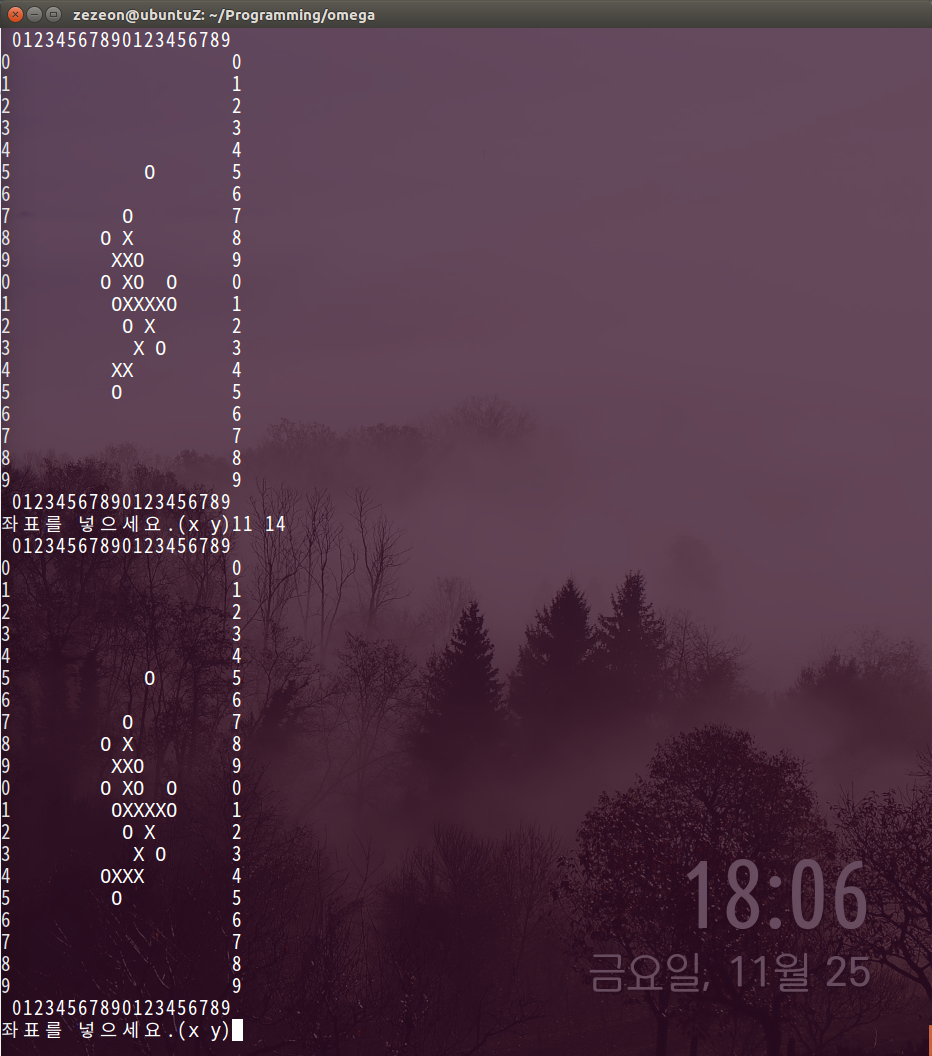
\includegraphics[width=\textwidth]{p.png}

프로그램의 실행은 실행파일명 뒤에 O, X 혹은 숫자의 옵션을 줄 수가 있다.
O를 줄 경우, 사람이 O를 잡는 것이고, X를 줄 경우 사람이 X를 잡는 것이다.
숫자를 옵션으로 줄 경우는 컴퓨터끼리 무작위 대전을 그 숫자의 판 만큼 하여 기보를 생성하는 것이다.

사람이 X로 둘 경우는 통계를 기반으로 하는 학습형 인공지능이 상대를 하고, 사람이 O를 둘 경우는 기본 주어진 룰 이외에는 컴퓨터끼리 둘 때처럼 랜덤하게 둔다.
비록 인공지능의 성능은 아직까지 시원찮으나 \textbf{랜덤과 비교해 보면 두 가지의 경우가 확실히 다른 것을 느낄 수 있다.}


\section{수행 결과에 대한 토의}
벼락치기도 학습이니만큼 어느 정도 인공지능을 형성했다고는 할 수 있다.
또한, 승패를 결정하는 수를 알아내는 것을 제외하면 아무런 알고리즘 없이 코딩을 끝까지 일관했으므로, 학습형이라는 것은 분명하다. 
성능 면에서는 미약하지만, 학습형이기에 발전의 가능성이 있다.
프로그램이 다루는 데이터가 많아서 기동에 매우 오랜 시간이 걸린다는 것은 큰 단점이다.


\section{기타}
만약 노트북이 아니라, 컴퓨터 자원이 많았다면, 지금 정도의 소스로도 충분히 인공지능을 만들어 낼 수도 있으리라 생각한다.
이 경우에는 오히려 일종의 통계적인 함정같은 것이 발생하리라 예측이 된다.
즉, 무작위의 경험에 의해 배우는 것이기에 한번 잘못된 데이터가 입력이 될 경우 인공지능이 계속 그런 식으로 두게 되는 것이다.
이럴 경우는 사람이 두어 줘서 여러번 이겨야 하는데, 사람이 가르칠 수 있는 판 수는 매우 제한적이다. 
그래서, 알파고의 경우도 명인들의 기보를 입력한다던가 하는 방식으로 인간의 고차원적인 사고 방식을 주입시켰던 것 같다. 
그렇게 본다면 인공지능이 완벽히 스스로 학습한다는 것은 먼 얘기인 것 같다.
결정적인 부분에서 인간에 의한 도움을 필요로 한다.

\chapter{부록}
소스코드 : 별첨
\end{document}
